\documentclass[main.tex]{subfiles}

\begin{document}

\newpage

\section{Chap 1: Introduction}

\subsection{V-SLAM}

SLAM = Simultaneous Localization and Mapping
\begin{itemize}
\item Localization = where am I?
\item Map building = what is the surrounding environment like?
\item e.g.: a moving rigid body, equipped with a specific sensor, estimates its motion and builds a model (certain kinds of description) of the surrounding environment, without a priori information. (In V-SLAM: sensor == camera)
\end{itemize}

Non-intrusive Sensors
\begin{itemize}
\item self-contained
\item hard, but can adapt to different environments
\item e.g. cameras, laser scanners, IMU
\end{itemize}

Intrusive sensors
\begin{itemize}
\item Depends on a prepared environments
\item easy, but not transferable
\item e.g. QR code, gliding rails
\end{itemize}

Cameras: monocular camera, stereo camera, RGB-D camera

Monocular camera
\begin{itemize}
\item + Captures photo (projection of 3D world to 2D plane)
\item + Simple to use
\item - no depth info
\begin{itemize}
	\item Soln: move the camera and estimate its motion, and distances + sizes of objects
	\item Pixel disparity: the movement of objects on the photo as the camera moves
\end{itemize}
\item - scale ambiguity
\begin{itemize}
	\item No clear solution
\end{itemize}
\item Human beings can use common-sense to determine depth from photo
\end{itemize}

Stereo camera = two monocular camera
\begin{itemize}
\item + Has depth info
\item + Applies to indoor \& outdoor
\item - Computational heavy
\item - Measuring distance is limited by baseline (the distance between two cameras) \& camera resolution
\item - Needs special calibration and configuration
\end{itemize}

RGB-D camera (aka depth camera)
\begin{itemize}
\item + Has depth info (measure distance by light travel time)
\item - narrow measurement range
\item - noisy data
\item - small field of view
\item - susceptibility to sunlight interference
\item - unable to measure transparent material
\end{itemize}

\subsection{Classical VSLAM Framework}

\begin{figure}[!h]
  \centering
  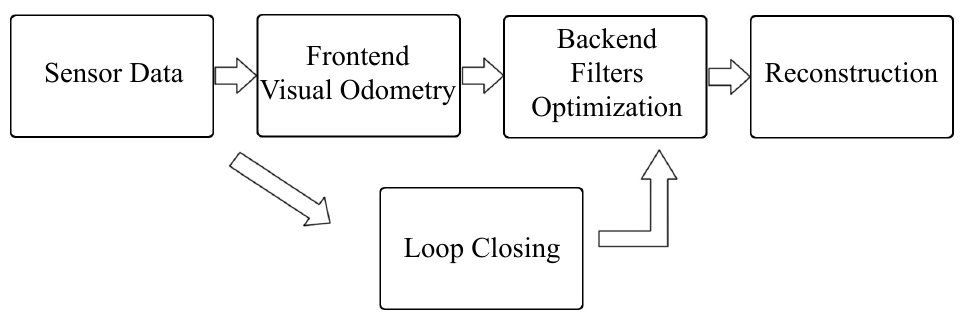
\includegraphics[width=0.6\linewidth]{vslam_framework.png}
  \caption{classic visual SLAM framework}
  \label{fig:vslam}
\end{figure}

\begin{itemize}
\item Sensor data acquisition: Camera images, motor encoders, IMU sensors etc
\item Visual Odometry (VO)
\begin{itemize}
	\item Estimate the camera movement between adjacent frames and generate a rough local map
	\item Wiki: visual odometry is the process of determining the position and orientation of a robot by analyzing the associated camera images
	\item Odometry = the use of data from motion sensors to estimate change in position over time
\end{itemize}
\item Filtering / Optimization: Generate a fully optimized trajectory and map
\item Loop Closing: Detect if the robot returned to previous position, to reduce the accumulated drift
\item Reconstruction: It constructs a task-specific map based on the estimated camera trajectory
\end{itemize}

\paragraph{VO}
Area: Computer Vision (CV), Image feature extraction \& matching

Prob: accumulative drift (propagated error)

Soln: backend optimization \& loop closing

In \href{https://www.mdpi.com/2218-6581/11/1/24}{A Comprehensive Survey of Visual SLAM Algorithms}, the authors mention VSLAM differs from VO by `the global consistency of the estimated trajectory and map' (rather than a belonging relationship in this book

\paragraph{Backend Optimization}
Area: State Estimation

Deal with noise

It studies (1) estimate camera movements; (2) noise in each estimation; (3) how noise is propagated; (4) how confident we have in the current estimation

Soln: Filtering, nonlinear optimization for estimating the mean and uncertainty (covariance) of the states

\paragraph{Loop Closing} aka loop closure detection
\begin{itemize}
\item Solving drifting problem in VO (correcting drifts accumulated at the end of the robot's trajectory)
\item E.g. of drifting: origin location != returned location
\item Need to enable robot to identify the scenes it has visited before
\item Intrusive methods: QR codes
\item Non-intrusive methods: visual loop detection (detect similarities between images; inspired by humans), laser-based SLAM
\end{itemize}

\paragraph{Mapping} the process of building a map (a description of the environment)
\begin{itemize}
\item Example of map: 2D grid map, 2D topological map, 3D point clouds, 3D meshes
\item The kind of map is highly dependent on the application
\item Metrical maps
\begin{itemize}
	\item emphasize the exact metrical locations of the objects in maps
	\item Sparse metric map: store the scene into a compact form, a partial form of the scene (Sufficient for localization task)
	\item Dense metric map: store all the things that are seen (Sufficient for localization and navigation task)
	\item Still have some open problems (wall overlapping due to steering error)
\end{itemize}
\item Topological maps
\begin{itemize}
	\item emphasize the relationships among map elements; consists of nodes \& edges, only considering the connectivity between nodes
	\item A more compact representation than metrical maps as we only consider connectivity
	\item Open problems: (1) How to split a map to form nodes and edges; (2) How to use a topological map for navigation \& path finding
\end{itemize}
\end{itemize}

\subsection{Mathematical Formulation of SLAM Problems}

\begin{itemize}
\item $\bx_i$: location of the robot at time step $i$
\item $\bx_1,\dots,\bx_k$: trajectory of the robot
\item $y$: landmark
\item $y_1,\dots,y_N$: total of N landmarks
\item motion: $\bx$ changes from step $k-1$ to step $k$
\item motion equation: $\bx_k = f(\bx_{k-1}, \bu_k, \bw_k)$, $\bu_k$ = input commands, $\bw_k$ = noise
\item observation: sees a landmark point $\by_j$ at $\bx_k$ and generates an observation data $\bz_{k,j}$
\item observation equation: $\bz_{k,j} = h(\by_j,\bx_k,\bv_{k,j})$
\end{itemize}

\bigskip
\begin{itemize}
\item pose = position + rotation (in this book)
\item The presence of noise makes the motion process stochastic: the robot will not move exactly as the command
\item Basic SLAM problem: how to solve the estimate $\bx$ (localization) and $\by$ (mapping) problem with the noisy control input $\bu$ and the sensor reading $\bz$ data?
\item SLAM problem is modeled as a \textit{state estimation problem}: How to estimate the internal, hidden state variables through the noisy measurement data?
\item State estimation problem is classified based on (non)-linearity of the observation equation, and the (non)-Gaussian noise.
\item Linear Gaussian (LG) system can be solved by Kalman Filter (KF)
\item Non-linear non-Gaussian (NLNG) can be solved by (1) Extended Kalman Filter (EKF); and (2) nonlinear optimization
\begin{itemize}
	\item SOTA: graph optimization
\end{itemize}
\end{itemize}



\end{document}